\chapter{Detection of a Measurement-Induced Phase Transition in Interacting Systems}
\thispagestyle{empty}
\label{chap:MIPT_bosons}

\section{Introduction}

\blfootnote{The content of this chapter consists of work done for a project which started in May 2019. Towards the final stages of finishing this project, we became aware of a preprint by Fuji et al., who independently were working on a very similar project \cite{fuji2020}. For this reason, we decided not to publish our work at the time. Furthermore, we concluded that with our limited system size data, we could not provide any strong claims regarding the precise location of the phase transition, which we will discuss in section \ref{subsec:discussion_scaling}.}

In chapter~\ref{chap:intro}, we introduced the measurement-induced phase transition (MIPT) that was discovered in random circuits \cite{li2018,li2019,skinner2019}, resulting from the competition between entangling unitary dynamics and disentangling local measurements. Qualitative changes in the system wave function characterize these phase transitions as the system undergoes a phase transition from volume-law to area-law scaling of the entropy at a critical measurement strength.

In this section, we study such MIPTs in continuous time systems at long times, which emerge from the competition between coherent time evolution and projective measurements that result from interactions with an environment. We explore a 1D chain of hard-core bosons that can tunnel between neighboring sites, and to break integrability, we include interactions between first and second neighbors. The system experiences on-site dephasing, which can be regarded as the result of an external observer performing projective measurements on the system and losing information to the environment. This could arise physically, for example, due to inelastic light scattering \cite{pichler2010,poletti2013,sarkar2014,luschen2017}. The model is discussed in more detail in the following section. The steady state of this model, at the density operator level, is the trivial infinite temperature state that is reached independent of the measurement strength, therefore masking the transition. To access the transition, we need to consider an unraveling of the master equation where we can study the entanglement properties. To achieve this, we use quantum trajectories and consider non-linear functions of the density operator, which are then averaged over individual measurement outcomes, which are no longer independent of measurement strength, thus revealing the transition.

We find that when the measurement strength is small, quantum correlations spanning the whole system are able to build up, and the volume-law scaling is preserved in the interacting model. For large measurement strengths, however, the system favors a product state where information becomes localized, and the entanglement does not build up. This provides an example of a system where the interplay between unitary and dissipative processes can fundamentally change the nature of the coherent dynamics, giving insights into how the entanglement properties of a system are affected by the coupling to an external reservoir. In the following sections, we will provide an analysis of the entropy scaling forms that emerge from this competition, perform finite size-scaling analysis, and provide conclusions that can be drawn from this analysis.

\section[Interacting Hard-Core Bosons and Free Fermions on a 1D Chain]{Interacting Hard-Core Bosons and Free \\ Fermions on a 1D Chain}

In this chapter, we study a chain of hard-core bosons that hop between neighboring sites, and we include first and second-neighbor interactions to break the integrability of the model. We simulate this model using exact diagonalization (ED) techniques, which heavily limits the system sizes we can access. We use the fact that in 1D, there is a one-to-one correspondence between a system consisting of hard-core bosons and spin-1/2 particles \cite{halperin1986}. Furthermore, spin-1/2 particles can be mapped to non-interacting free fermions via the Jordan-Wigner transformation \cite{nielsen}, 
\begin{align}
\begin{split}    
    \hat{\sigma}_j^+ &= \hat{c}_j^\dagger K_j^+, \\
    \hat{\sigma}_j^- &= \hat{c}_j K_j^-, \\
    \hat{\sigma}_j^z &= \hat{c}_j^\dagger \hat{c}_j - \frac{1}{2},
\end{split}
\end{align}
where $\hat{K}_j^{\pm} = e^{\pm i \pi \sum_{k<j} \hat{n}_k}$ is the string operator, with $n_k = \hat{c}_j^\dagger \hat{c}_i$ the fermionic number operator in site $j$, and $\hat{c}_j^\dagger, \hat{c}_j$ the creation and annihilation operators respectively in site $j$.
This transformation allows us to compare our results in a bosonic system with those in a fermionic system. Free fermions enable efficient simulation of much larger system sizes at the cost of being restricted to only being able to consider the non-interacting case. Nevertheless, this still is a powerful tool that allows us to draw valuable conclusions in this chapter.

\subsection{Model I}
    \begin{figure}[ht]
        \centering
        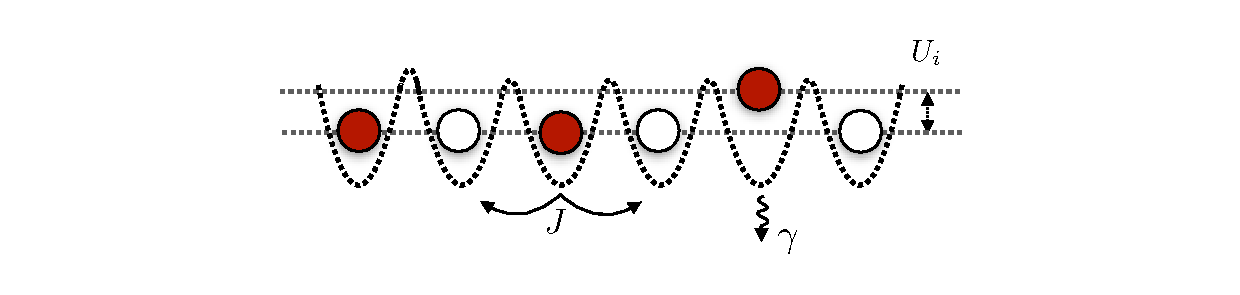
\includegraphics[width = \textwidth]{Chapters/Plots/Chapter4/Chapter3_Fig1.pdf}
        \caption{Schematic representation of a periodic 1D system consisting of hard-core bosons, subject to dissipation. $J$ describes the hopping strength, $U_i$ describes the interaction strength between sites at a distance $i$ and $\gamma$ describes the dissipation strength. We assume periodic boundary conditions, $M+1\equiv 1$, where $M$ is the number of lattice sites.}
        \label{fig:Chapter3_Fig1}
    \end{figure}
    
We consider a periodic 1D chain (Fig.~\ref{fig:Chapter3_Fig1}) that consists of hard-core bosons (particles that cannot occupy the same state, i.e., we have at most one particle per site) with nearest-neighbor hopping and interactions between first and second neighbors to break integrability, described by the system Hamiltonian,
\begin{equation}
\hat{H} =  \hat{H}^b_\text{hop} + \hat{H}_\text{int}.
\end{equation}
The term $\hat{H}^b_\text{hop}$ describes the hopping Hamiltonian,
\begin{equation}
\label{eq:ham}
\hat{H}^b_\text{hop} =-J \sum\limits_{i=1}^{M} ( \hat{a}^{\dagger}_i \hat{a}_{i+1} + \textrm{h.c.}),
\end{equation}
with hopping parameter $J$.  $\hat{a}^\dagger_i, \hat{a}_i$ are the respective bosonic creation and annihilation operators in sites $i$, satisfying the commutation relations, $[a_i,a_j^\dagger] = \delta_{ij}$ and $[a_i,a_j]= [a_i^\dagger, a_j^\dagger] = 0$.

The second term denotes the interaction Hamiltonian,
\begin{equation}
\hat{H}_\text{int} = U_1\sum\limits_{i=1}^{M} \hat{n}_i \hat{n}_{i+1}
+ U_2\sum\limits_{i=1}^{M} \hat{n}_i \hat{n}_{i+2},
\end{equation}
where $U_1$, and $U_2$ are the interaction strengths between first and second neighbors respectively and $\hat{n}_i=\hat{a}_i^\dagger \hat{a}_i$. 

For simulating the dynamics of the fermionic system, we replace the bosonic operators in the Hamiltonian described in Eq.~\ref{eq:ham}, with the fermionic raising and lowering operators, $\hat{c}^\dagger_i, \hat{c}_i$,
\begin{equation}
\hat{H}^f_\text{hop} =-J \sum\limits_{i=1}^{M} ( \hat{c}^{\dagger}_i \hat{c}_{i+1} + \textrm{h.c.}).
\end{equation}
The fermionic operators satisfy the anticommutation relations, $\{c_i,c_j^\dagger\} = \delta_{ij}$ and $\{c_i,c_j\}= \{c_i^\dagger, c_j^\dagger\} = 0$, where $\{a,b\} \equiv ab + ba$ defines the anticommutator.

For both hard-core bosons and FGS, we consider this system subject to dephasing of the local particle numbers, with the number operator $\hat{n}_i$ being the jump operator that models the dissipation. The system dynamics are described by the GKSL master equation (Eq.~\ref{eq:GKSL_meq}). We consider a photon counting unraveling of the master equation to simulate the dynamics and access the phase transition. Due to the conservation of the $U(1)$ symmetry in the model, we can explicitly compute the jump times from Eq.~\ref{eq:jumptime} using $t_{i+1} = -\dfrac{\ln{r}}{\gamma N}$, where $\gamma$ is the measurement strength, $N$ is the total particle number, and $r$ is a random number drawn uniformly from the interval $(0,1)$.

\subsection{Model II}
\label{subsec:model2}
To explore in more detail what can be deduced from Model I, we turn to the secondary model, which consists of the same Hamiltonian, but we substitute the dephasing process with a single particle pump and loss term. We do this to explicitly break the $U(1)$ symmetry associated with excitation number conservation. The resulting GKSL master equation reads, 
\begin{equation}
\label{eq:meqpm}
    \dot{\hat{\rho}} = -i [\hat{H},\hat{\rho}] + \gamma^+ \sum\limits_i \Big[ \hat{a}^{\dagger}_i \hat{\rho} \hat{a}_i -\frac{1}{2} \{\hat{a}_i\hat{a}^{\dagger}_i, \hat{\rho}\} \Big] + \gamma^- \sum\limits_i \Big[ \hat{a}_i \hat{\rho} \hat{a}^{\dagger}_i -\frac{1}{2} \{\hat{a}^{\dagger}_i\hat{a}_i, \hat{\rho}\}\Big],
\end{equation}
where $\gamma^+, \gamma^-$ are the new dissipation strengths that describe the pump and loss processes. The jump operators associated with the pump and loss terms are the creation $\hat{a}_i^\dagger$ and annihilation operators $\hat{a}_i$, respectively. As we would like to ensure the stationary state remains the infinite temperature state $\mathbb{I}/d$, where $d$ is the system dimension. Noting that in the stationary state $\dot{\hat{\rho}} = 0$, substituting $\rho=
\mathbb{I}/d$ in Eq.~\ref{eq:meqpm} and multiplying by $d$ we obtain, 
\begin{align}
\begin{split}
    -i [\hat{H},\mathbb{I}] + \gamma^+ \sum\limits_i \Big[ \hat{a}^{\dagger}_i \mathbb{I} \hat{a}_i -\frac{1}{2} \{\hat{a}_i\hat{a}^{\dagger}_i, \mathbb{I}\} \Big] + \gamma^- \sum\limits_i \Big[ \hat{a}_i \mathbb{I} \hat{a}^{\dagger}_i -\frac{1}{2} \{\hat{a}^{\dagger}_i\hat{a}_i, \mathbb{I}\}\Big] &= 0\\
    \gamma^+ \sum\limits_i \Big[ \hat{a}^{\dagger}_i \hat{a}_i - \hat{a}_i\hat{a}^{\dagger}_i \Big] + \gamma^- \sum\limits_i \Big[ \hat{a}_i \hat{a}^{\dagger}_i - \hat{a}^{\dagger}_i\hat{a}_i\Big] &= 0 \\
    (\gamma^+-\gamma^-) \sum\limits_i ( \hat{a}^{\dagger}_i\hat{a}_i - \hat{a}_i \hat{a}^{\dagger}_i) &= 0 \\
    (\gamma^+-\gamma^-) \sum\limits_i [\hat{a}_i, \hat{a}^{\dagger}_i] &= 0
\end{split}
\end{align}
As $[\hat{a}_i, \hat{a}^{\dagger}_i] = 1$, we deduce that in order to ensure that the stationary state remains the infinite temperature state, we must choose $\gamma^+ = \gamma^-$. 

\section{Non-interacting vs. interacting systems}

We will begin by analyzing the long-time entanglement properties for both the interacting and non-interacting models to find evidence of a dynamical phase transition between volume-law and area-law scaling of the entanglement entropy as a function of the dissipation strength. We explore whether: i) there are distinguishable phases in which the entanglement properties are qualitatively different, ii) there is a quantum critical point $\gamma_c$ at which the system undergoes a dynamical phase transition. We will shortly show that although the behavior in the interacting model clearly allows us to see different entanglement properties, especially in the regimes far from the transition point, pinpointing the critical point is a difficult task. Due to the finite-size systems explored here, the critical point cannot be extracted with certainty from this data, which is the topic of discussion in subsection \ref{subsec:discussion_scaling}. 

To obtain the data presented in this chapter, we make use of higher-order quantum trajectories and follow the procedure discussed in chapter \ref{subsec:higher_order}. To ensure that we have reached the stationary regime, we time-evolve until the trajectory averaged local densities stop oscillating and reach an approximately steady value. When the stationary regime is reached, we compute the trajectory average of the von Neumann entropy \cite{nielsen2000} as a function of the subsystem size. The von Neumann entropy is defined as,
\begin{equation}
    S(M_A) = -\Tr [\hat{\rho}_{A} \ln\hat{\rho}_{A}],
\end{equation}
where $\hat{\rho}_{A} = \Tr_B(\hat{\rho})$ is the reduced density operator of a subset $M_A \in [1,M-1]$ of the full system consisting of $M$ sites and $B$ denotes the remainder of the system.

    \begin{figure}[ht]
        \centering
        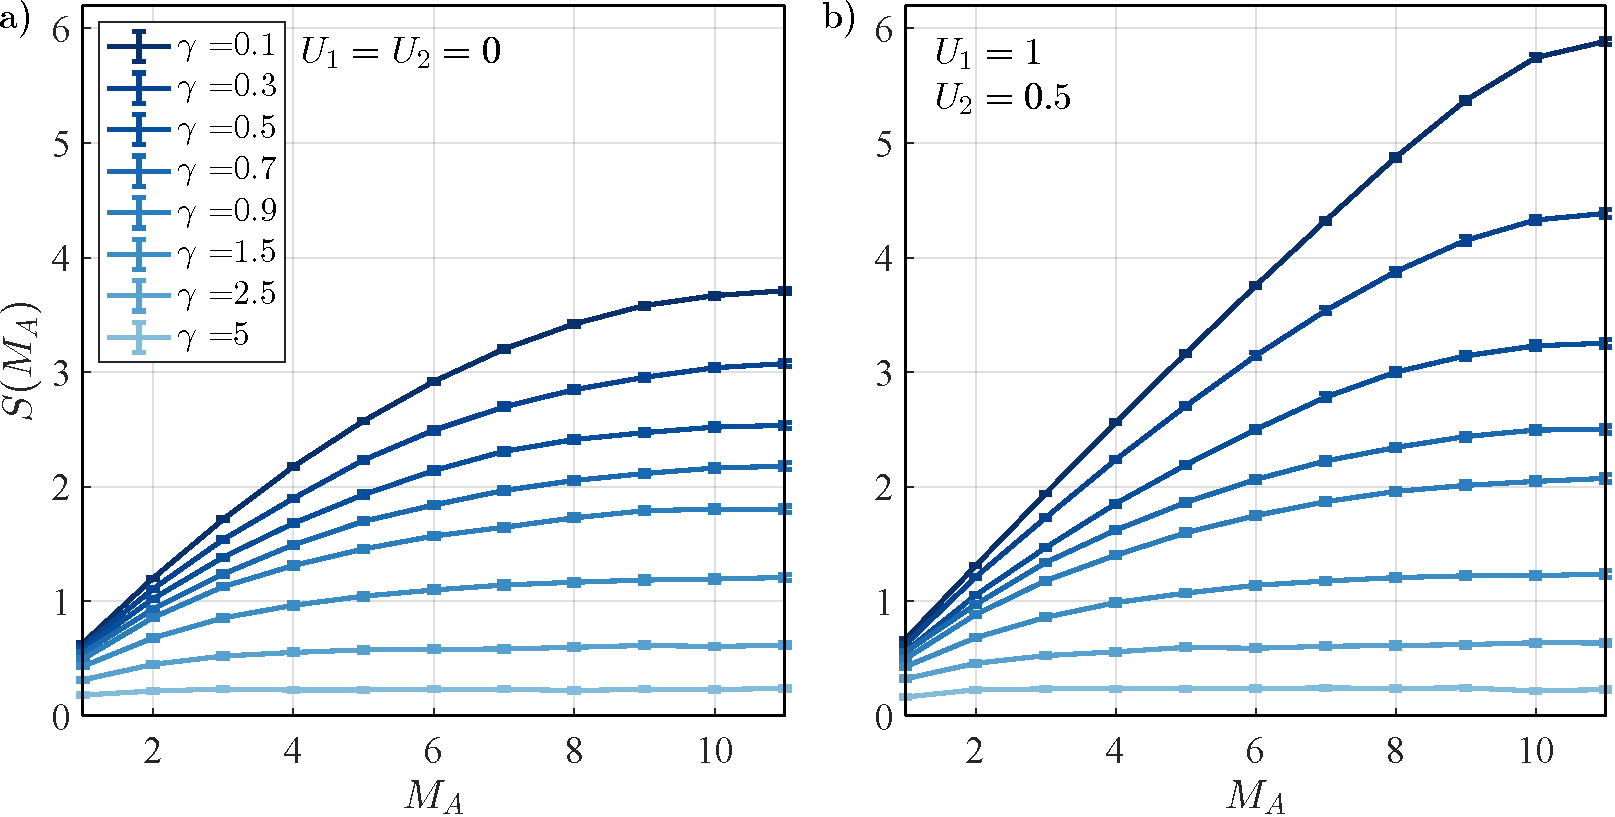
\includegraphics[width=\textwidth]{Chapters/Plots/Chapter4/Chapter3_Fig2.pdf}
        \caption{The von Neumann entropy $S(M_A)$ of the approximate stationary state as a function of subsystem size $M_A$ ($M=22$) for a) the non-interacting model $U_1 = U_2 = 0$, and b) the interacting model with $U_1 = 1, U_2 = 0.5$. A range of dissipation strengths is presented, $\gamma \in [0.1,0.3,0.5,0.7,0.9,1.5,2.5,5]$, visualized in dark to light blue. We time-evolve until ~$TJ = 60$ and compute trajectory averages using $N_t = 300$ trajectories. The statistical error bars are computed using $\sigma = \sigma_S / \sqrt{N_t}$, where $\sigma_S$ is the standard deviation of the data. As both plots highlight, the statistical error bars are small, and we observe good convergence. The legend presented in a) also applies to b).}
        \label{fig:Chapter3_Fig2}
    \end{figure}

In Fig.~\ref{fig:Chapter3_Fig2} b), we can see that the entropy displays significantly qualitatively different behavior for small and large $\gamma$ in the interacting model. For small $\gamma$, we see volume-law scaling, characterized by linear growth of the entropy with subsystem size. In contrast, for large $\gamma$, we see that the entanglement entropy remains invariant under the increase of the subsystem size, suggesting area-law scaling. In the volume-law phase, we see that as $M_A \to M/2$, the linear growth starts to curve, showing some logarithmic corrections to the linear growth, as seen in Ref.~\cite{fuji2020}. Even in these relatively small systems, there appears to be a clear transition between volume-law scaling and area-law scaling of the entropy. In contrast, in Fig.~\ref{fig:Chapter3_Fig2} a), in the non-interacting model for small $\gamma$, the entropy only grows logarithmically, is then fully suppressed in the area-law regime and remains constant as a function of subsystem size. The transition between logarithmic scaling and area-law scaling is present in both models and seems to occur around similar dissipation strengths. To characterize the change between these three distinct behavioral patterns, we can fit a function consisting of a linear, a logarithmic, and a constant term,
\begin{equation}
    f(x) = a x + b \ln{x} + c,
\end{equation}
and investigate how the fitting parameters vary with the dissipation strengths. 

\begin{figure}[ht]
    \centering
    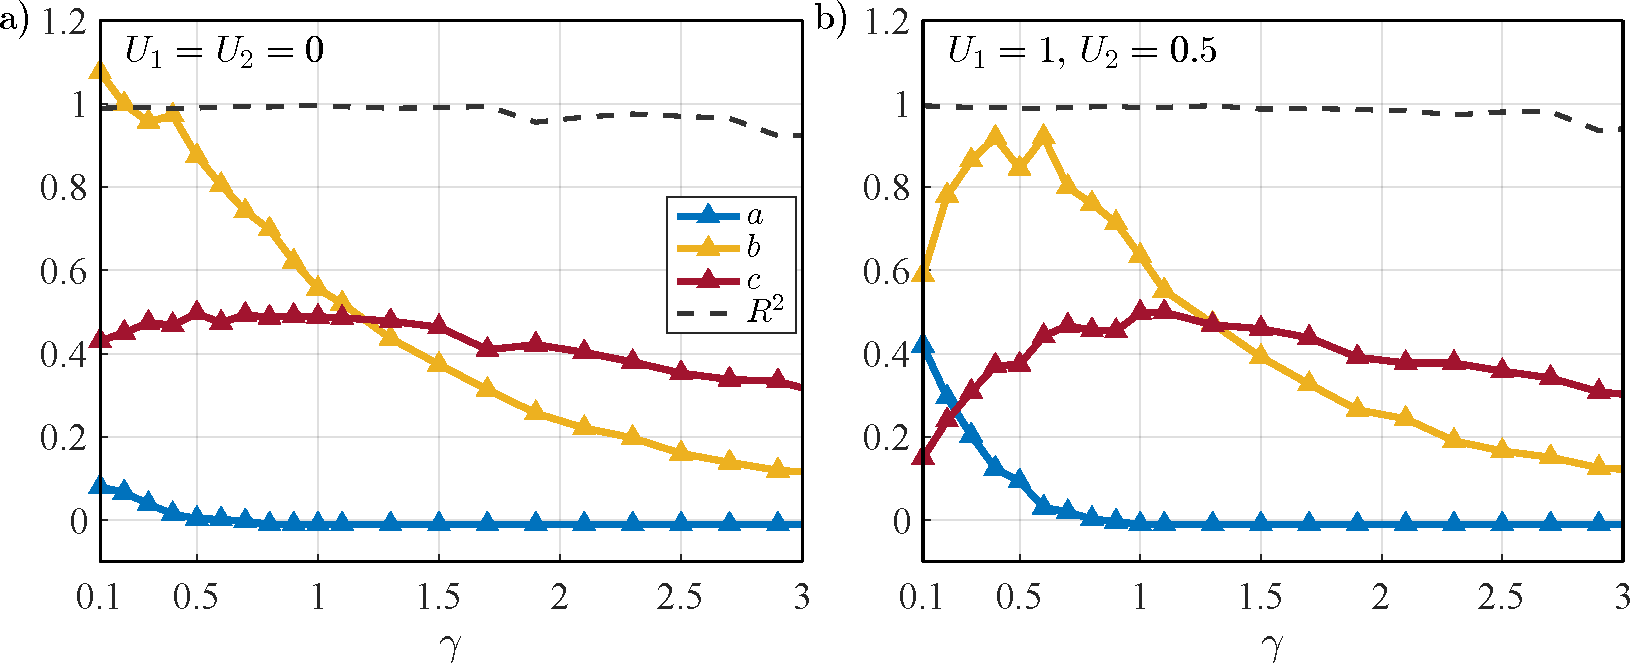
\includegraphics[width=\textwidth]{Chapters/Plots/Chapter4/Chapter3_Fig3.pdf}
    \caption{We plot the coefficients of the fitting function $f(x) = a x + b \ln{x} + c$ as a function of the dissipation strength $\gamma \in [0.1, 3]$ to analyze which terms dominate in which regimes, for a) the non-interacting model and b) the interacting model. The dotted line shows the coefficient of determination $R^2$ close to 1, indicating a good fit for the data. The function $f(x)$ was fitted to the data with $M = 22$ sites to limit the finite-size effects as much as possible. The legend presented in a) also applies to b). Due to the low statistical error bars in Fig.~\ref{fig:Chapter3_Fig2}, we can be confident that the fits we have obtained are accurate. All system parameters are identical to the ones presented in Fig.~\ref{fig:Chapter3_Fig2}}
    \label{fig:Chapter3_Fig3}
\end{figure}

From Fig.~\ref{fig:Chapter3_Fig3}, we can guess where the transition points might lie by analyzing where the different coefficients dominate the scaling behavior. Firstly we can see a clear difference in the linear coefficient $a$. It only plays a small role in the non-interacting case, whereas in the interacting model, we can see a larger contribution matching the behavior we have seen for small $\gamma$ in Fig.~\ref{fig:Chapter3_Fig3}. Secondly, the logarithmic coefficient $b$ dominates the scaling of the entropy in the non-interacting model for small $\gamma$. It continuously decreases with increasing dissipation strength, while in the interacting model, it first grows until $a \approx 0$. Then it also decreases continuously with a similar trend as in the non-interacting model. The constant term $c$ fluctuates around $0.5$ in the non-interacting model while it increases until $\gamma = 1$, and then the qualitative behavior of $c$ appears to be the same in both models. We learn from this figure that there seem to be two regimes for the two models, one in which the fitting coefficients behave differently and one where they appear to exhibit the same trends. While $\gamma<1$, we see significant differences in the fitting parameters between the two models, which is what we would expect as the non-interacting model does not have a volume-law phase while the interacting model does. Then as we have already seen in Fig.~\ref{fig:Chapter3_Fig2}, the transition point between logarithmic and area-law scaling seems to occur around the same dissipation strength, which seems to be in the range $\gamma \in [1,2]$, as this is the regime in which $c$ remains approximately constant, while $b$ continuously approaches $0$. Our data suggests that in the interacting model, a transition between volume-law and logarithmic scaling occurs near $\gamma = 1$, while in both models, a transition appears from logarithmic scaling to area-law scaling on the interval $\gamma \in [1,2]$. Furthermore, the scaling forms of the entropy in the interacting case seem to follow a linear trend with logarithmic corrections and a constant term, and as we approach $\gamma = 1$ the linear term vanishes. After that, logarithmic scaling of the entropy with a constant term describes the behavior of the entropy in the interacting and non-interacting cases.

This analysis provides estimates of which regimes of the parameter space to look for a scaling collapse of the data, also referred to as data collapse. This means rather than considering one single system size to find the transition point; we simulate a range of system sizes and \textit{collapse} all of our data onto a single curve to gain insight into the critical parameters of the transition using a standard scaling form which we introduce below. To further investigate this, we plot the von Neumann entropy in Fig.~\ref{fig:Chapter3_Fig4} between two equally sized subsystems $M_A = M/2$ for a variety of system sizes as a function of the dissipation strength $\gamma$.

\begin{figure}[ht]
    \centering
    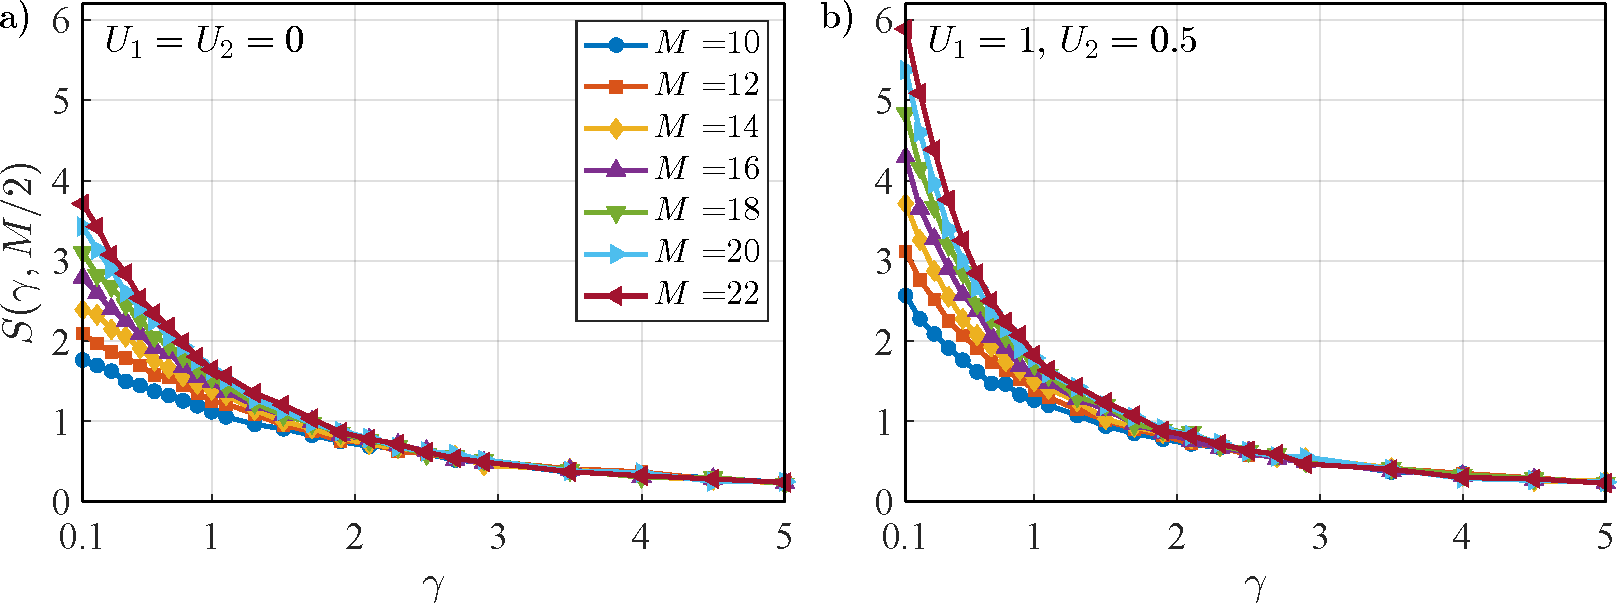
\includegraphics[width=\textwidth]{Chapters/Plots/Chapter4/Chapter3_Fig4.pdf}
    \caption{We plot the trajectory-averaged approximate steady-state von Neumann entropy in the middle bipartition as a function of dissipation strength $\gamma$ for various system sizes. Numerical parameters remain as described in Fig.~\ref{fig:Chapter3_Fig2}. As before, we plot the a) non-interacting case, $U_1 = U_2 = 0$, and b) interacting case $U_1 = 1, U_2 = 0.5$. The legend presented in a) also applies to b).}
    \label{fig:Chapter3_Fig4}
\end{figure}
This plot clearly shows the data begins to collapse in the regime $\gamma \in [1,2]$ for the non-interacting and interacting cases. This is the regime we associate with the transition to area-law scaling; however, this figure reveals no indication regarding a transition from volume-law scaling to logarithmic scaling. Moreover, this figure demonstrates the difficulty of highlighting an exact transition point where the volume-law phase ends, which is most likely due to the limited system sizes we have been able to access in our calculations. We dedicate the next section to the closer examination of this problem by looking at finite size scalings proposed in the literature \cite{skinner2019} and explain the conclusions we draw from our data and calculations.
 
\section{Discussion of scaling collapses}
\label{subsec:discussion_scaling}

In this section, we attempt to pinpoint the critical points at which the transitions between the different regimes occur. As mentioned in the introduction, near criticality, quantum systems are said to be \textit{scale-invariant}. We, therefore, expect that some continuous function describes the behavior of the entropy at criticality, independent of the total system size. In general, we cannot simulate infinitely large systems, which is why we consider a range of accessible system sizes and perform finite size scaling to extract the critical point and exponents. 

From our analysis, we expect the entropy in the vicinity of the critical point to behave as $S(\gamma,M_A) \sim c \ln(M_A)$, where $c$ is a constant. We introduce a scaling function $G(M/\xi)$, where $M$ is the system size and $\xi \sim |\gamma - \gamma_c|^{-\nu}$ describes the correlation length for the critical exponent $\nu$. With this scaling function, we can write, 
\begin{equation}
\label{eq:scalingG}
    S(\gamma,M_A) = c \ln(M_A) + G(M |\gamma - \gamma_c|^{-\nu}).
\end{equation}
By subtracting the entropy at the critical point $S(\gamma_c, M_A)$, we can rewrite Eq.~\ref{eq:scalingG} as,
\begin{equation}
    S(\gamma,M/2) - S(\gamma_c,M/2) = F((\gamma - \gamma_c) M^{1/\nu}), 
\end{equation}
where $F$ is a different scaling function than before, $S(\gamma,M/2)$ is the von Neumann entropy in the steady state between two equal subsystems ($M_A = M/2$) for a dissipation strength $\gamma$ and $\nu$ is the critical exponent associated to the correlation length $\xi \sim |\gamma - \gamma_c|^{-\nu}$.

When $\gamma_c$ and $\nu$ are known, this form can then easily be verified by plotting $S(\gamma,M/2) - S(\gamma_c,M/2)$ as a function of $(\gamma - \gamma_c) M^{1/\nu}$ for a range of system sizes, and all simulated data points should collapse onto a single curve. As in our case, we do not know $\nu$ and have only estimates for $\gamma_c$ we can use this Ansatz to search for the optimal collapse parameters which should pinpoint the transition point. This Ansatz also has been used in related works \cite{skinner2019, fuji2020, li2019} in random circuit models and continuous-time systems.

We now provide a brief overview of the algorithm used to search for the optimal collapse parameters; the full outline is provided in Ref.\cite{skinner2019}. First we define the parameters, $x = (\gamma - \gamma_c) M^{1/\nu}$ and $y(x) = S(\gamma,M/2) - S(\gamma_c,M/2)$. Using spline interpolation for all simulated system sizes, we estimate $S(\gamma_c,M/2)$ for a given estimate $\gamma_c$. We then compute $x$ and $y(x)$ for all simulated parameters $\gamma$ and $M$ in the dataset. This results in a family of curves, and we obtain the optimal scaling parameters by minimizing the mean-square deviation from their mains for any given point $x_i$. All points $x_i$ that lie outside the range of simulated values for $x$ are discarded.

The application of this algorithm to our data has shown scaling collapses for multiple parameter combinations. We expect to see a data collapse at the critical point where we change from one regime into the other. Only the interacting model exhibits a volume-law phase, and from Fig.~\ref{fig:Chapter3_Fig3}~b), we expect that the transition occurs close to where the linear term of the fitting function vanishes, which is the case around $\gamma_c \approx 1$. 

\begin{figure}[ht]
    \centering
    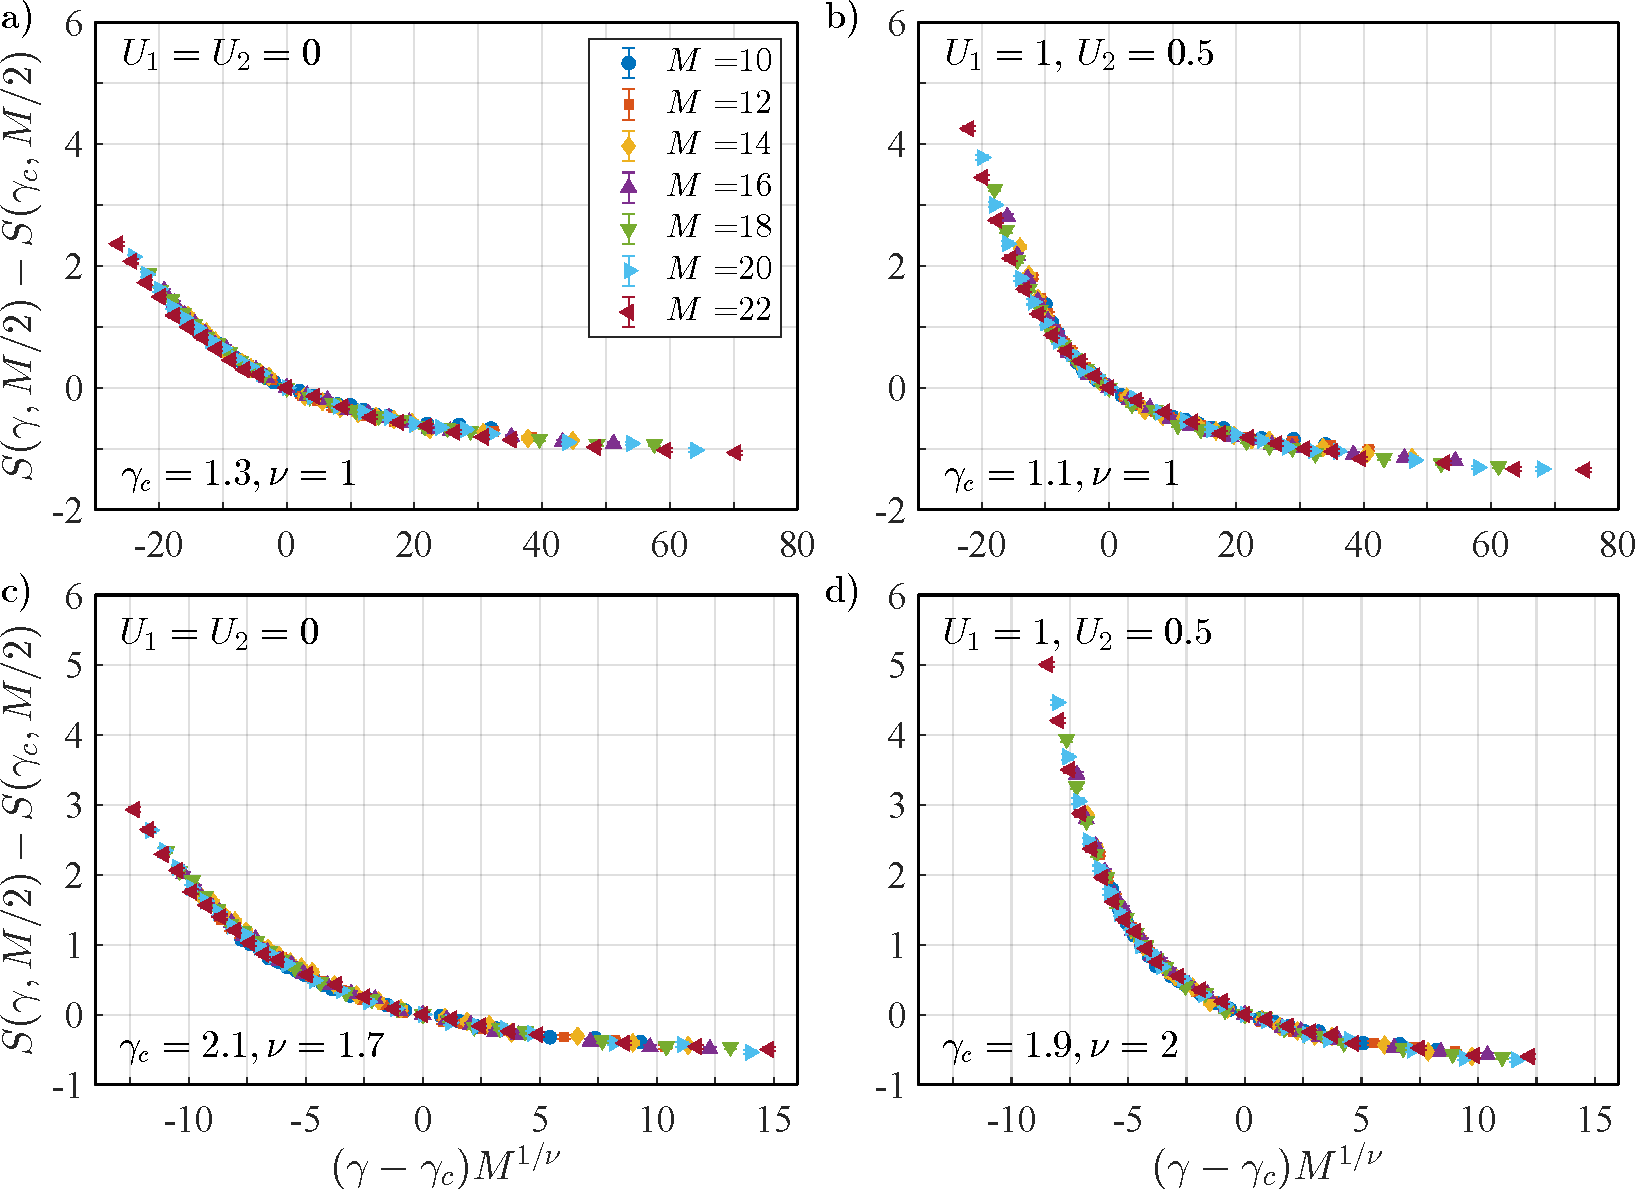
\includegraphics[width=\textwidth]{Chapters/Plots/Chapter4/Chapter3_Fig5.pdf}
    \caption{Scaling collapse of the data from Fig.~\ref{fig:Chapter3_Fig4}, for a) the non-interacting integrable model, and b) the interacting non-integrable model. The scaling parameters depicted here are a) $\gamma_c = 1.3, \nu = 1$, b) $\gamma_c = 1.1, \nu = 1$, c) $\gamma_c = 2.1, \nu = 1.7$, and d) $\gamma_c = 1.9, \nu = 2$. The legend presented in a) also applies to b)-d).}
    \label{fig:Chapter3_Fig5}
\end{figure}

In Fig.~\ref{fig:Chapter3_Fig5}~a)-b) we plot the data collapse in a) the non-interacting model with critical dissipation rate $\gamma_c = 1.3$, and b) in the interacting model with critical dissipation rate $\gamma_c = 1.1$ and $\nu = 1$ in both models. These parameters are obtained by minimizing a cost function, and the resulting scaling collapses are presented here. The critical dissipation rates we have obtained here match our estimates $\gamma \approx 1$, for the volume-law transition. In the non-interacting model, we also see a data collapse for a similar dissipation rate. This is surprising as we do not expect this to happen as this model does not exhibit a volume-law phase. Other parameter values for which the cost function of the search algorithm is minimal could be found, which we have displayed in Fig.~\ref{fig:Chapter3_Fig5}~c)-d). These parameter values match our estimates, where we expect the transition from logarithmic to area-law scaling for $\gamma \approx 2$. As this behavior is present in both models here, we would expect to see a data collapse in both models. 

Furthermore, we found that it was possible to obtain collapses for other parameter values in the non-interacting model. This means that although we observe the transition in the entanglement entropy, we are not able to pinpoint the critical dissipation rates exactly, as we are able to collapse the data for a variety of parameter values, suggesting that the system sizes that we have explored here are not large enough. 

To test whether the system size is the issue, we use Fermionic Gaussian States (FGS) and consider a 1D-chain of free fermions. The non-interacting model we have considered is described by a quadratic Hamiltonian, which allows us to efficiently simulate larger systems consisting of free fermions using the methods introduced in chapter~\ref{sec:FGS}. We simulate the same system sizes that we explored for the hard-core bosons, perform a data collapse, and then add larger system sizes to see whether the data collapse remains unchanged. 

\begin{figure}[ht]
    \centering
    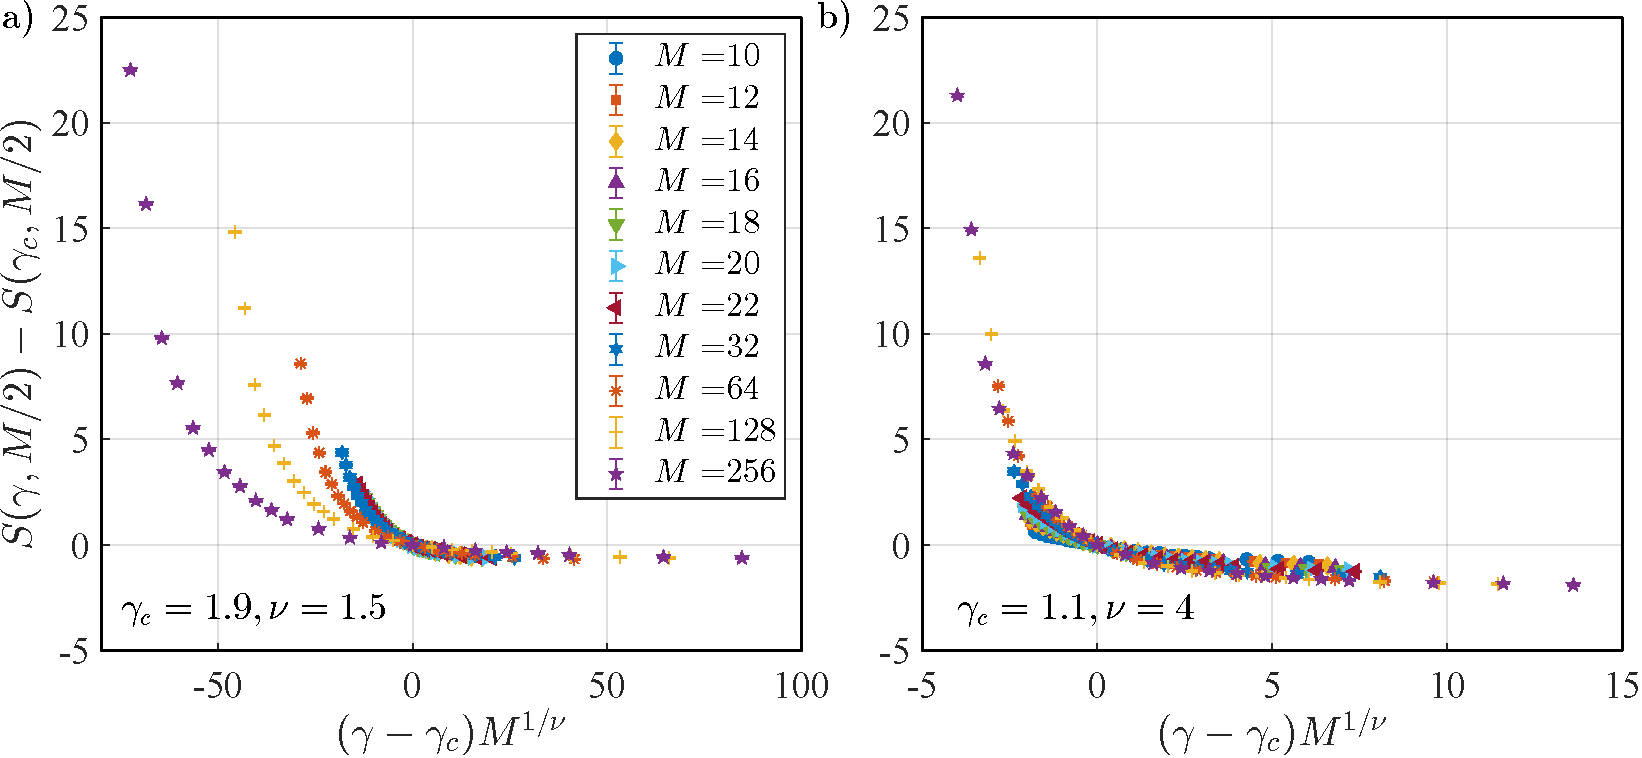
\includegraphics[width=\textwidth]{Chapters/Plots/Chapter4/Chapter3_Fig6.pdf}
    \caption{Scaling collapse of the von Neumann entropy in the fermionic system. In a), we use system sizes $M \leq 32$ to search for optimal collapse parameters; in b), we use the system sizes $M \geq 64$. We then plot the resulting data collapse for all the parameters. The depicted scaling parameters are a) $\gamma_c = 1.9, \nu = 1.5$, and b) $\gamma_c = 1.1, \nu = 4$. The legend presented in a) also applies to b).}
    \label{fig:Chapter3_Fig6}
\end{figure}

Fig.~\ref{fig:Chapter3_Fig6}~a) shows the data collapse when we only include system sizes $M \leq 32$ in the data set. We find that $\gamma_c = 1.9, \nu = 1.5$ leads to the optimal data collapse. This plot clearly shows, however, that the scaling collapse does not work for larger system sizes, which means the system sizes in the data set are simply too small. Furthermore, if we use the large system sizes and perform a data collapse, depicted in Fig.~\ref{fig:Chapter3_Fig6}~b), we see a much better data collapse, where the smaller system sizes follow the trend of the larger ones. 

In this section, we have demonstrated that we can clearly distinguish the different regimes by plotting the entropy as a function of system size; however, we cannot make definitive claims about where the transition points lie when we can only access relatively small system sizes. We have observed large deviations in the scaling collapses when including and excluding certain system sizes for the free fermion model. Moreover, for the hard-core boson data, we expect a data collapse for the interacting model at small measurement strengths but do not expect one in the non-interacting model. Fig.~\ref{fig:Chapter3_Fig5}~a), b), however, shows data collapses for similar collapse parameters in the interacting and non-interacting model, irrespective of whether or not we expect a data collapse to occur. We conclude that we cannot trust the data collapses and critical parameters we extract from a data set if it only contains data for small system sizes.

\section{Breaking the \texorpdfstring{$U(1)$}~~symmetry: single pump and loss}

In this section, we will focus on Model II as described in section~\ref{subsec:model2}. Instead of considering a local dephasing process, we introduce single-particle pump and loss in the system. In Model I, we conserve the $U(1)$ symmetry associated with the total particle number conservation. By considering single pump and loss processes, with respective strengths, $\gamma^+$, and $\gamma^-$, we explicitly break the particle number conservation to explore whether we can witness and pinpoint the transition. For the remainder of this section, we will only consider the case $\gamma^\pm = \gamma^+ = \gamma^-$ to ensure the steady state remains the infinite temperature state with average particle number $M/2$. 

\begin{figure}[hbt!]
    \centering
    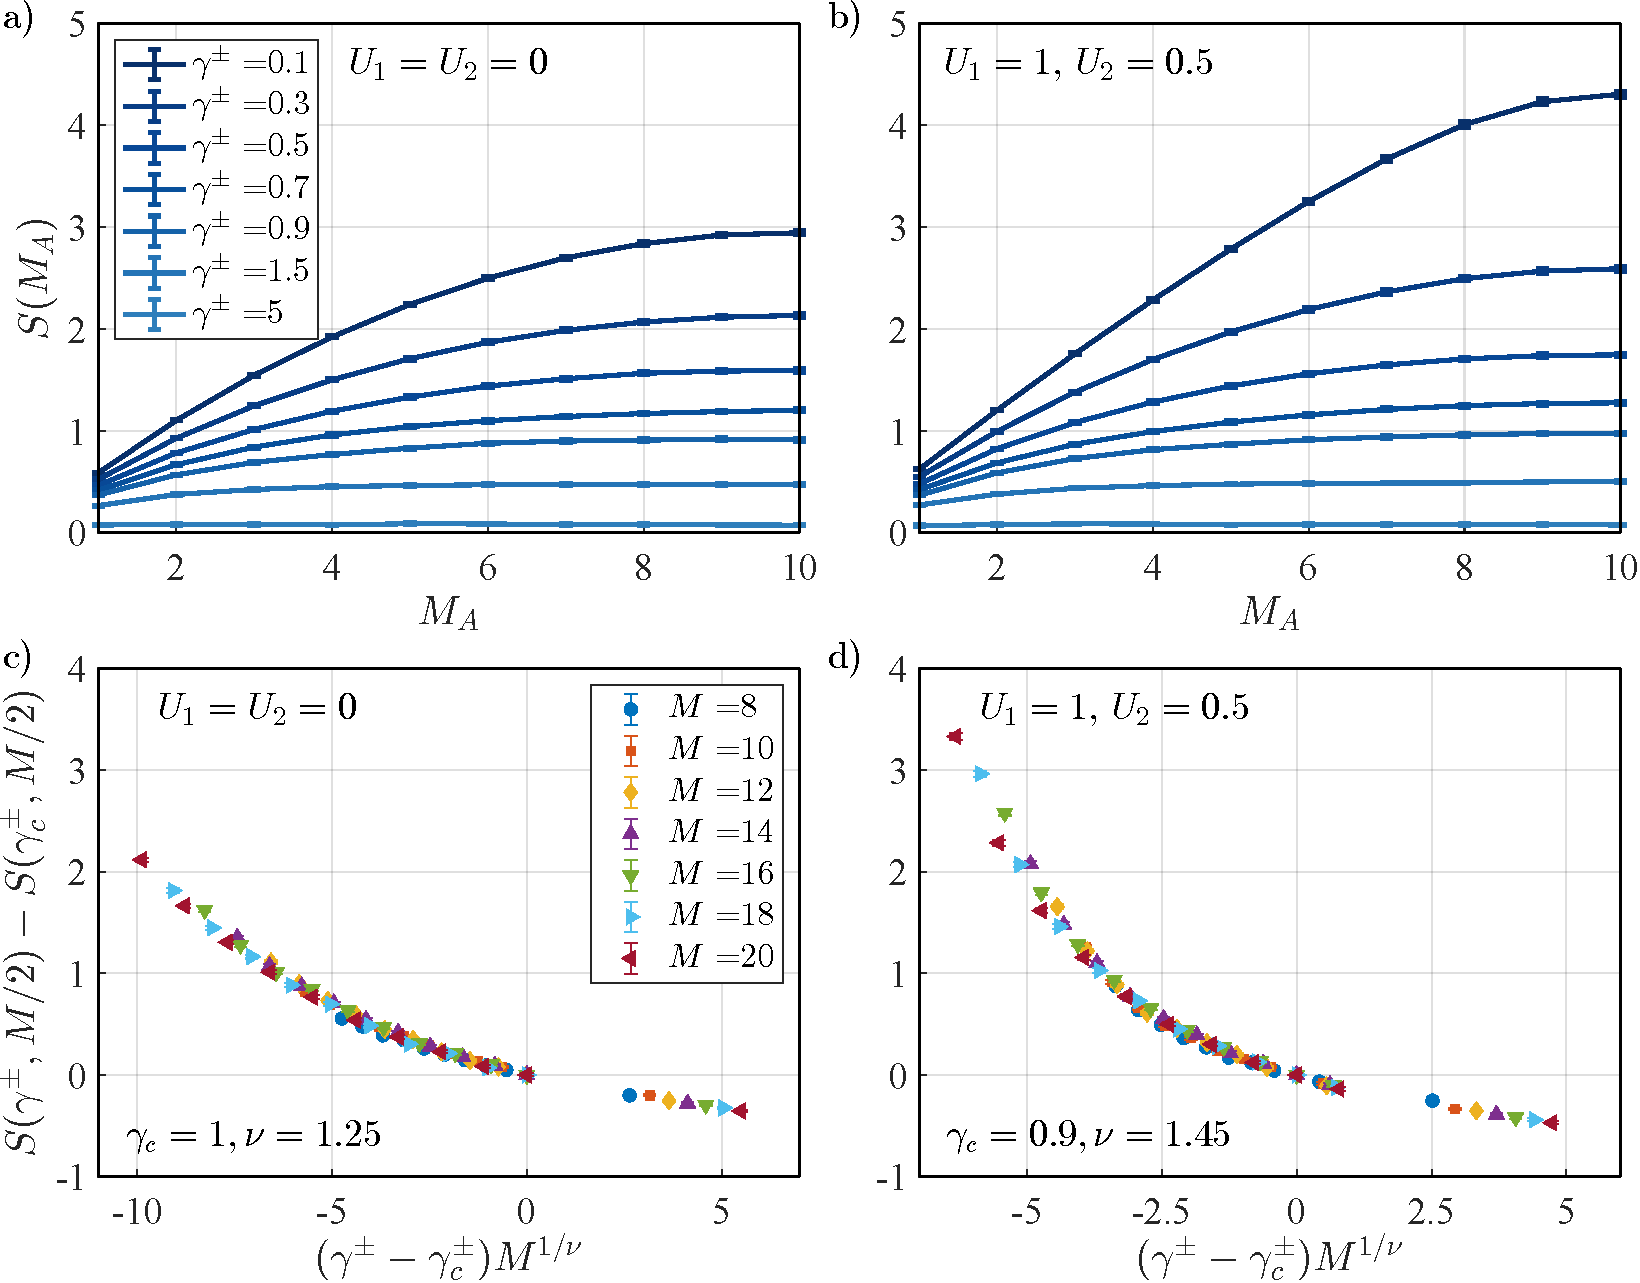
\includegraphics[width=0.99\textwidth]{Chapters/Plots/Chapter4/Chapter3_Fig7.pdf}
    \caption{a)-b) The von Neumann entropy of the approximate stationary state as a function of subsystem size $M_A$ ($M=20$) for a) the non-interacting model $U_1 = U_2 = 0$, and b) the interacting model with $U_1 = 1, U_2 = 0.5$. We time-evolve until $TJ = 60$ and compute trajectory averages using $N_t = 300$ trajectories. The legend presented in a) also applies to b). c)-d) Scaling collapse of the data from a)-b) for the non-interacting and interacting models, respectively. The statistical error bars for a) and b) were calculated in the same fashion as in Fig.~\ref{fig:Chapter3_Fig2} and are sufficiently small, indicating good convergence. The scaling parameters depicted here are c) $\gamma^\pm_c = 1, \nu = 1.25$, and d) $\gamma^\pm_c = 0.9, \nu = 1.45$.}
    \label{fig:Chapter3_Fig7}
\end{figure}

In Fig.~\ref{fig:Chapter3_Fig7}~a)-b), we plot the von Neumann entropy for the non-interacting and interacting models, respectively. As before, we witness volume-law scaling of the entropy in the interacting model for small dissipation strengths $\gamma^\pm$, characterized by linear growth of the entropy with subsystem size. Moreover, as for Model I, we witness a logarithmic regime, which then transitions into an area-law phase where the entropy is constant. We see that there are no qualitative differences in the behavior of the entropy when compared to the case of dephasing despite explicitly breaking the $U(1)$ symmetry. Although we clearly see different signatures in the behavior of the entropy, it is difficult to pinpoint the exact transition point. In Fig~\ref{fig:Chapter3_Fig7}~c)-d), we plot the scaling collapses of the von Neumann entropy of the bipartition, $M_A = [1, M/2]$, for the optimal scaling parameters. Again, we see a similar situation as before: similar critical dissipation strength and exponents collapse the data. In addition, we found other parameters that also collapsed the data, further proving that the accessible system sizes were not sufficiently large to pinpoint the critical point exactly. 

\section{Conclusion}

In this chapter, we have explored the dynamical phase transition that arises due to the competition between coherent time evolution and disentangling dissipative processes such as dephasing and single particle pump and loss. We have seen that we can clearly distinguish between different regimes characterized by the behavior of the entanglement entropy. When using standard methods to extract critical parameters to reveal the transition points, we find that scaling collapses can appear regardless of whether a transition occurs. We have seen that for similar critical parameters, we see data collapses in the bosonic system in both the interacting and non-interacting models, which is concerning since we do not see a transition from volume-law to logarithmic scaling of the entropy in the non-interacting model. We are limited to moderate system sizes ($M \sim 20$) that we can simulate using exact diagonalization, and we do not have the same tools as in random circuits where efficient algorithms exist for system sizes that are an order of magnitude larger ($M \sim 10^2$). 

For the non-interacting model, we also considered a system of free fermions, where we simulated the same system sizes as for the bosonic system but also included larger system sizes, up to $M = 256$. This allowed us to assess the quality of the data collapse we witnessed in the bosonic system by considering different subsets of the system sizes. We first only used small system sizes to obtain a data collapse, which drastically changed upon including the large system sizes to extract the collapse parameters. Furthermore, the collapse parameters we extracted using only the small system sizes do not collapse the larger ones. We, therefore, conclude from this analysis that it is difficult to pinpoint the transition point precisely when we only have access to small system sizes, and we cannot necessarily trust the collapse results when only considering small system sizes, as we did in the bosonic case.

We further explored a system consisting of hard-core bosons, described by the same Hamiltonian but with a single particle pump and loss term, and found qualitatively the same behavior in the entanglement entropy and distinct regimes. Similarly, as for the first model, we see again that scaling collapses appear whether or not a transition occurs, resulting in the conclusion that the accessible system sizes we have been able to explore are too small to make exact claims regarding the precise location of the critical points at which the transitions occur. 

A natural approach to simulate larger system sizes would be to write the system wave function as a matrix product state, which could efficiently represent the state in the area-law regime. In the volume-law regime, however, we could not efficiently represent the system wave function as the truncation to low bond dimensions in the matrix product state relies on working with states that only have moderate or small amounts of entanglement. This clearly is not the case in the volume-law regime, making this not a suitable solution for this problem. 

In the following chapters, we will continue to explore the competition between unitary and dissipative dynamics that give rise to MIPTs. We explore questions regarding the experimental detection of such dynamical phase transitions in chapter~\ref{chap:MIPT_continuous_measurement} and our efforts to find observables that witness the transition that would be experimentally feasible. In chapter~\ref{chap:short_time_dynamics}, we explore whether we can find evidence of different regimes when considering the short-time dynamics as we have only explored the behavior of the stationary states. We further explore whether we can find a feasible method of revealing the transition in an experiment. 
